\documentclass[1p]{elsarticle_modified}
%\bibliographystyle{elsarticle-num}

%\usepackage[colorlinks]{hyperref}
%\usepackage{abbrmath_seonhwa} %\Abb, \Ascr, \Acal ,\Abf, \Afrak
\usepackage{amsfonts}
\usepackage{amssymb}
\usepackage{amsmath}
\usepackage{amsthm}
\usepackage{scalefnt}
\usepackage{amsbsy}
\usepackage{kotex}
\usepackage{caption}
\usepackage{subfig}
\usepackage{color}
\usepackage{graphicx}
\usepackage{xcolor} %% white, black, red, green, blue, cyan, magenta, yellow
\usepackage{float}
\usepackage{setspace}
\usepackage{hyperref}

\usepackage{tikz}
\usetikzlibrary{arrows}

\usepackage{multirow}
\usepackage{array} % fixed length table
\usepackage{hhline}

%%%%%%%%%%%%%%%%%%%%%
\makeatletter
\renewcommand*\env@matrix[1][\arraystretch]{%
	\edef\arraystretch{#1}%
	\hskip -\arraycolsep
	\let\@ifnextchar\new@ifnextchar
	\array{*\c@MaxMatrixCols c}}
\makeatother %https://tex.stackexchange.com/questions/14071/how-can-i-increase-the-line-spacing-in-a-matrix
%%%%%%%%%%%%%%%

\usepackage[normalem]{ulem}

\newcommand{\msout}[1]{\ifmmode\text{\sout{\ensuremath{#1}}}\else\sout{#1}\fi}
%SOURCE: \msout is \stkout macro in https://tex.stackexchange.com/questions/20609/strikeout-in-math-mode

\newcommand{\cancel}[1]{
	\ifmmode
	{\color{red}\msout{#1}}
	\else
	{\color{red}\sout{#1}}
	\fi
}

\newcommand{\add}[1]{
	{\color{blue}\uwave{#1}}
}

\newcommand{\replace}[2]{
	\ifmmode
	{\color{red}\msout{#1}}{\color{blue}\uwave{#2}}
	\else
	{\color{red}\sout{#1}}{\color{blue}\uwave{#2}}
	\fi
}

\newcommand{\Sol}{\mathcal{S}} %segment
\newcommand{\D}{D} %diagram
\newcommand{\A}{\mathcal{A}} %arc


%%%%%%%%%%%%%%%%%%%%%%%%%%%%%5 test

\def\sl{\operatorname{\textup{SL}}(2,\Cbb)}
\def\psl{\operatorname{\textup{PSL}}(2,\Cbb)}
\def\quan{\mkern 1mu \triangleright \mkern 1mu}

\theoremstyle{definition}
\newtheorem{thm}{Theorem}[section]
\newtheorem{prop}[thm]{Proposition}
\newtheorem{lem}[thm]{Lemma}
\newtheorem{ques}[thm]{Question}
\newtheorem{cor}[thm]{Corollary}
\newtheorem{defn}[thm]{Definition}
\newtheorem{exam}[thm]{Example}
\newtheorem{rmk}[thm]{Remark}
\newtheorem{alg}[thm]{Algorithm}

\newcommand{\I}{\sqrt{-1}}
\begin{document}

%\begin{frontmatter}
%
%\title{Boundary parabolic representations of knots up to 8 crossings}
%
%%% Group authors per affiliation:
%\author{Yunhi Cho} 
%\address{Department of Mathematics, University of Seoul, Seoul, Korea}
%\ead{yhcho@uos.ac.kr}
%
%
%\author{Seonhwa Kim} %\fnref{s_kim}}
%\address{Center for Geometry and Physics, Institute for Basic Science, Pohang, 37673, Korea}
%\ead{ryeona17@ibs.re.kr}
%
%\author{Hyuk Kim}
%\address{Department of Mathematical Sciences, Seoul National University, Seoul 08826, Korea}
%\ead{hyukkim@snu.ac.kr}
%
%\author{Seokbeom Yoon}
%\address{Department of Mathematical Sciences, Seoul National University, Seoul, 08826,  Korea}
%\ead{sbyoon15@snu.ac.kr}
%
%\begin{abstract}
%We find all boundary parabolic representation of knots up to 8 crossings.
%
%\end{abstract}
%\begin{keyword}
%    \MSC[2010] 57M25 
%\end{keyword}
%
%\end{frontmatter}

%\linenumbers
%\tableofcontents
%
\newcommand\colored[1]{\textcolor{white}{\rule[-0.35ex]{0.8em}{1.4ex}}\kern-0.8em\color{red} #1}%
%\newcommand\colored[1]{\textcolor{white}{ #1}\kern-2.17ex	\textcolor{white}{ #1}\kern-1.81ex	\textcolor{white}{ #1}\kern-2.15ex\color{red}#1	}

{\Large $\underline{11a_{132}~(K11a_{132})}$}

\setlength{\tabcolsep}{10pt}
\renewcommand{\arraystretch}{1.6}
\vspace{1cm}\begin{tabular}{m{100pt}>{\centering\arraybackslash}m{274pt}}
\multirow{5}{120pt}{
	\centering
	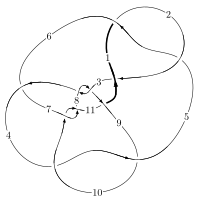
\includegraphics[width=112pt]{../../../GIT/diagram.site/Diagrams/png/381_11a_132.png}\\
\ \ \ A knot diagram\footnotemark}&
\allowdisplaybreaks
\textbf{Linearized knot diagam} \\
\cline{2-2}
 &
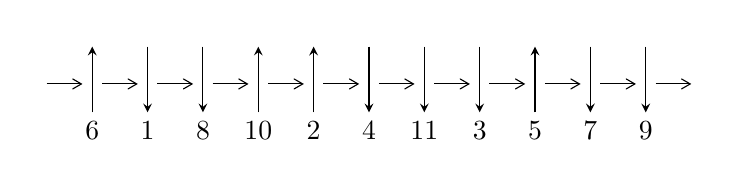
\begin{tikzpicture}[x=20pt, y=17pt]
	% nodes
	\node (C0) at (0, 0) {};
	\node (C1) at (1, 0) {};
	\node (C1U) at (1, +1) {};
	\node (C1D) at (1, -1) {6};

	\node (C2) at (2, 0) {};
	\node (C2U) at (2, +1) {};
	\node (C2D) at (2, -1) {1};

	\node (C3) at (3, 0) {};
	\node (C3U) at (3, +1) {};
	\node (C3D) at (3, -1) {8};

	\node (C4) at (4, 0) {};
	\node (C4U) at (4, +1) {};
	\node (C4D) at (4, -1) {10};

	\node (C5) at (5, 0) {};
	\node (C5U) at (5, +1) {};
	\node (C5D) at (5, -1) {2};

	\node (C6) at (6, 0) {};
	\node (C6U) at (6, +1) {};
	\node (C6D) at (6, -1) {4};

	\node (C7) at (7, 0) {};
	\node (C7U) at (7, +1) {};
	\node (C7D) at (7, -1) {11};

	\node (C8) at (8, 0) {};
	\node (C8U) at (8, +1) {};
	\node (C8D) at (8, -1) {3};

	\node (C9) at (9, 0) {};
	\node (C9U) at (9, +1) {};
	\node (C9D) at (9, -1) {5};

	\node (C10) at (10, 0) {};
	\node (C10U) at (10, +1) {};
	\node (C10D) at (10, -1) {7};

	\node (C11) at (11, 0) {};
	\node (C11U) at (11, +1) {};
	\node (C11D) at (11, -1) {9};
	\node (C12) at (12, 0) {};

	% arrows
	\draw[->,>={angle 60}]
	(C0) edge (C1) (C1) edge (C2) (C2) edge (C3) (C3) edge (C4) (C4) edge (C5) (C5) edge (C6) (C6) edge (C7) (C7) edge (C8) (C8) edge (C9) (C9) edge (C10) (C10) edge (C11) (C11) edge (C12) ;	\draw[->,>=stealth]
	(C1D) edge (C1U) (C2U) edge (C2D) (C3U) edge (C3D) (C4D) edge (C4U) (C5D) edge (C5U) (C6U) edge (C6D) (C7U) edge (C7D) (C8U) edge (C8D) (C9D) edge (C9U) (C10U) edge (C10D) (C11U) edge (C11D) ;
	\end{tikzpicture} \\
\hhline{~~} \\& 
\textbf{Solving Sequence} \\ \cline{2-2} 
 &
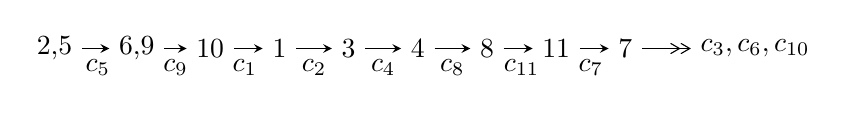
\begin{tikzpicture}[x=25pt, y=7pt]
	% node
	\node (A0) at (-1/8, 0) {2,5};
	\node (A1) at (17/16, 0) {6,9};
	\node (A2) at (17/8, 0) {10};
	\node (A3) at (25/8, 0) {1};
	\node (A4) at (33/8, 0) {3};
	\node (A5) at (41/8, 0) {4};
	\node (A6) at (49/8, 0) {8};
	\node (A7) at (57/8, 0) {11};
	\node (A8) at (65/8, 0) {7};
	\node (C1) at (1/2, -1) {$c_{5}$};
	\node (C2) at (13/8, -1) {$c_{9}$};
	\node (C3) at (21/8, -1) {$c_{1}$};
	\node (C4) at (29/8, -1) {$c_{2}$};
	\node (C5) at (37/8, -1) {$c_{4}$};
	\node (C6) at (45/8, -1) {$c_{8}$};
	\node (C7) at (53/8, -1) {$c_{11}$};
	\node (C8) at (61/8, -1) {$c_{7}$};
	\node (A9) at (10, 0) {$c_{3},c_{6},c_{10}$};

	% edge
	\draw[->,>=stealth]	
	(A0) edge (A1) (A1) edge (A2) (A2) edge (A3) (A3) edge (A4) (A4) edge (A5) (A5) edge (A6) (A6) edge (A7) (A7) edge (A8) ;
	\draw[->>,>={angle 60}]	
	(A8) edge (A9);
\end{tikzpicture} \\ 

\end{tabular} \\

\footnotetext{
The image of knot diagram is generated by the software ``\textbf{Draw programme}" developed by Andrew Bartholomew(\url{http://www.layer8.co.uk/maths/draw/index.htm\#Running-draw}), where we modified some parts for our purpose(\url{https://github.com/CATsTAILs/LinksPainter}).
}\phantom \\ \newline 
\centering \textbf{Ideals for irreducible components\footnotemark of $X_{\text{par}}$} 
 
\begin{align*}
I^u_{1}&=\langle 
-116 u^{48}-310 u^{47}+\cdots+2304 b-8416,\;-4487 u^{49}-19250 u^{48}+\cdots+71424 a-445724,\\
\phantom{I^u_{1}}&\phantom{= \langle  }u^{50}+4 u^{49}+\cdots+255 u+62\rangle \\
I^u_{2}&=\langle 
b^2- b u+u,\;a- u+1,\;u^2- u+1\rangle \\
I^u_{3}&=\langle 
b+u,\;a-2,\;u^2- u+1\rangle \\
I^u_{4}&=\langle 
b^2 a u+b^3+b u+a u+b+u-1,\;u^2- u+1\rangle \\
\\
I^v_{1}&=\langle 
a,\;b^3+b-1,\;v-1\rangle \\
\end{align*}
\raggedright * 4 irreducible components of $\dim_{\mathbb{C}}=0$, with total 59 representations.\\
\raggedright * 1 irreducible components of $\dim_{\mathbb{C}}=1$ \\
\footnotetext{All coefficients of polynomials are rational numbers. But the coefficients are sometimes approximated in decimal forms when there is not enough margin.}
\newpage
\renewcommand{\arraystretch}{1}
\centering \section*{I. $I^u_{1}= \langle -116 u^{48}-310 u^{47}+\cdots+2304 b-8416,\;-4487 u^{49}-19250 u^{48}+\cdots+71424 a-445724,\;u^{50}+4 u^{49}+\cdots+255 u+62 \rangle$}
\flushleft \textbf{(i) Arc colorings}\\
\begin{tabular}{m{7pt} m{180pt} m{7pt} m{180pt} }
\flushright $a_{2}=$&$\begin{pmatrix}0\\u\end{pmatrix}$ \\
\flushright $a_{5}=$&$\begin{pmatrix}1\\0\end{pmatrix}$ \\
\flushright $a_{6}=$&$\begin{pmatrix}1\\- u^2\end{pmatrix}$ \\
\flushright $a_{9}=$&$\begin{pmatrix}0.0628220 u^{49}+0.269517 u^{48}+\cdots+24.7408 u+6.24054\\0.0503472 u^{48}+0.134549 u^{47}+\cdots+9.09288 u+3.65278\end{pmatrix}$ \\
\flushright $a_{10}=$&$\begin{pmatrix}0.0628220 u^{49}+0.319864 u^{48}+\cdots+33.8336 u+9.89331\\0.0503472 u^{48}+0.134549 u^{47}+\cdots+9.09288 u+3.65278\end{pmatrix}$ \\
\flushright $a_{1}=$&$\begin{pmatrix}- u\\u^3+u\end{pmatrix}$ \\
\flushright $a_{3}=$&$\begin{pmatrix}- u^3\\u^5+u^3+u\end{pmatrix}$ \\
\flushright $a_{4}=$&$\begin{pmatrix}0.0753528 u^{49}+0.332661 u^{48}+\cdots+20.5942 u+5.51184\\0.0104167 u^{49}+0.0559896 u^{48}+\cdots+3.65495 u+0.393229\end{pmatrix}$ \\
\flushright $a_{8}=$&$\begin{pmatrix}0.176103 u^{49}+0.671427 u^{48}+\cdots+38.7086 u+8.87769\\0.0625000 u^{49}+0.159722 u^{48}+\cdots+4.80382 u+1.71528\end{pmatrix}$ \\
\flushright $a_{11}=$&$\begin{pmatrix}-0.0727487 u^{49}-0.228495 u^{48}+\cdots-18.8299 u-4.29049\\0.0625000 u^{49}+0.190104 u^{48}+\cdots+3.84115 u-0.151042\end{pmatrix}$ \\
\flushright $a_{7}=$&$\begin{pmatrix}0.0408546 u^{49}+0.0874636 u^{48}+\cdots-6.34781 u-1.55343\\0.0156250 u^{49}-0.0447049 u^{48}+\cdots-12.4293 u-3.52170\end{pmatrix}$\\ \flushright $a_{7}=$&$\begin{pmatrix}0.0408546 u^{49}+0.0874636 u^{48}+\cdots-6.34781 u-1.55343\\0.0156250 u^{49}-0.0447049 u^{48}+\cdots-12.4293 u-3.52170\end{pmatrix}$\\&\end{tabular}
\flushleft \textbf{(ii) Obstruction class $= -1$}\\~\\
\flushleft \textbf{(iii) Cusp Shapes $= \frac{625}{864} u^{49}+\frac{5359}{1728} u^{48}+\cdots+\frac{43991}{216} u+\frac{193}{4}$}\\~\\
\newpage\renewcommand{\arraystretch}{1}
\flushleft \textbf{(iv) u-Polynomials at the component}\newline \\
\begin{tabular}{m{50pt}|m{274pt}}
Crossings & \hspace{64pt}u-Polynomials at each crossing \\
\hline $$\begin{aligned}c_{1},c_{5}\end{aligned}$$&$\begin{aligned}
&u^{50}+4 u^{49}+\cdots+255 u+62
\end{aligned}$\\
\hline $$\begin{aligned}c_{2}\end{aligned}$$&$\begin{aligned}
&u^{50}+20 u^{49}+\cdots+27851 u+3844
\end{aligned}$\\
\hline $$\begin{aligned}c_{3},c_{8}\end{aligned}$$&$\begin{aligned}
&9(9 u^{50}+9 u^{49}+\cdots-6 u+1)
\end{aligned}$\\
\hline $$\begin{aligned}c_{4},c_{9}\end{aligned}$$&$\begin{aligned}
&9(9 u^{50}+9 u^{49}+\cdots+8 u+1)
\end{aligned}$\\
\hline $$\begin{aligned}c_{6}\end{aligned}$$&$\begin{aligned}
&16(16 u^{50}-32 u^{49}+\cdots-26298 u+5463)
\end{aligned}$\\
\hline $$\begin{aligned}c_{7},c_{10}\end{aligned}$$&$\begin{aligned}
&u^{50}-6 u^{49}+\cdots-7031 u+1274
\end{aligned}$\\
\hline $$\begin{aligned}c_{11}\end{aligned}$$&$\begin{aligned}
&16(16 u^{50}-16 u^{49}+\cdots+612 u+63)
\end{aligned}$\\
\hline
\end{tabular}\\~\\
\newpage\renewcommand{\arraystretch}{1}
\flushleft \textbf{(v) Riley Polynomials at the component}\newline \\
\begin{tabular}{m{50pt}|m{274pt}}
Crossings & \hspace{64pt}Riley Polynomials at each crossing \\
\hline $$\begin{aligned}c_{1},c_{5}\end{aligned}$$&$\begin{aligned}
&y^{50}+20 y^{49}+\cdots+27851 y+3844
\end{aligned}$\\
\hline $$\begin{aligned}c_{2}\end{aligned}$$&$\begin{aligned}
&y^{50}+20 y^{49}+\cdots+97271135 y+14776336
\end{aligned}$\\
\hline $$\begin{aligned}c_{3},c_{8}\end{aligned}$$&$\begin{aligned}
&81(81 y^{50}+2457 y^{49}+\cdots-2 y+1)
\end{aligned}$\\
\hline $$\begin{aligned}c_{4},c_{9}\end{aligned}$$&$\begin{aligned}
&81(81 y^{50}+2781 y^{49}+\cdots-2 y+1)
\end{aligned}$\\
\hline $$\begin{aligned}c_{6}\end{aligned}$$&$\begin{aligned}
&256(256 y^{50}-1408 y^{49}+\cdots-8.62735\times10^{7} y+2.98444\times10^{7})
\end{aligned}$\\
\hline $$\begin{aligned}c_{7},c_{10}\end{aligned}$$&$\begin{aligned}
&y^{50}-34 y^{49}+\cdots+15979843 y+1623076
\end{aligned}$\\
\hline $$\begin{aligned}c_{11}\end{aligned}$$&$\begin{aligned}
&256(256 y^{50}-1920 y^{49}+\cdots+153522 y+3969)
\end{aligned}$\\
\hline
\end{tabular}\\~\\
\newpage\flushleft \textbf{(vi) Complex Volumes and Cusp Shapes}
$$\begin{array}{c|c|c}  
\text{Solutions to }I^u_{1}& \I (\text{vol} + \sqrt{-1}CS) & \text{Cusp shape}\\
 \hline 
\begin{aligned}
u &= \phantom{-}0.092353 + 1.013550 I \\
a &= -0.004651 - 0.358199 I \\
b &= \phantom{-}0.717415 + 0.391005 I\end{aligned}
 & -2.36463 + 4.68098 I & -6.72560 - 6.42701 I \\ \hline\begin{aligned}
u &= \phantom{-}0.092353 - 1.013550 I \\
a &= -0.004651 + 0.358199 I \\
b &= \phantom{-}0.717415 - 0.391005 I\end{aligned}
 & -2.36463 - 4.68098 I & -6.72560 + 6.42701 I \\ \hline\begin{aligned}
u &= -0.777689 + 0.592166 I \\
a &= \phantom{-}1.48088 + 0.63093 I \\
b &= -1.077960 - 0.011537 I\end{aligned}
 & \phantom{-}3.41598 + 5.21199 I & \phantom{-}0.12705 - 3.56799 I \\ \hline\begin{aligned}
u &= -0.777689 - 0.592166 I \\
a &= \phantom{-}1.48088 - 0.63093 I \\
b &= -1.077960 + 0.011537 I\end{aligned}
 & \phantom{-}3.41598 - 5.21199 I & \phantom{-}0.12705 + 3.56799 I \\ \hline\begin{aligned}
u &= -0.813463 + 0.649972 I \\
a &= -1.136810 - 0.407519 I \\
b &= \phantom{-}0.746378 - 0.288180 I\end{aligned}
 & \phantom{-}6.17950 + 0.24137 I & \phantom{-}3.95341 + 1.60515 I \\ \hline\begin{aligned}
u &= -0.813463 - 0.649972 I \\
a &= -1.136810 + 0.407519 I \\
b &= \phantom{-}0.746378 + 0.288180 I\end{aligned}
 & \phantom{-}6.17950 - 0.24137 I & \phantom{-}3.95341 - 1.60515 I \\ \hline\begin{aligned}
u &= \phantom{-}0.736653 + 0.765266 I \\
a &= -0.584317 - 1.167250 I \\
b &= \phantom{-}0.120988 + 1.046830 I\end{aligned}
 & -3.34886 + 2.77656 I & -9.46596 - 3.37700 I \\ \hline\begin{aligned}
u &= \phantom{-}0.736653 - 0.765266 I \\
a &= -0.584317 + 1.167250 I \\
b &= \phantom{-}0.120988 - 1.046830 I\end{aligned}
 & -3.34886 - 2.77656 I & -9.46596 + 3.37700 I \\ \hline\begin{aligned}
u &= \phantom{-}0.941593 + 0.502895 I \\
a &= \phantom{-}0.691476 - 0.854824 I \\
b &= -0.51438 + 1.34602 I\end{aligned}
 & -0.83094 - 10.80580 I & -3.00000 + 5.61837 I \\ \hline\begin{aligned}
u &= \phantom{-}0.941593 - 0.502895 I \\
a &= \phantom{-}0.691476 + 0.854824 I \\
b &= -0.51438 - 1.34602 I\end{aligned}
 & -0.83094 + 10.80580 I & -3.00000 - 5.61837 I\\
 \hline 
 \end{array}$$\newpage$$\begin{array}{c|c|c}  
\text{Solutions to }I^u_{1}& \I (\text{vol} + \sqrt{-1}CS) & \text{Cusp shape}\\
 \hline 
\begin{aligned}
u &= \phantom{-}0.447528 + 0.991757 I \\
a &= \phantom{-}0.195342 + 1.153440 I \\
b &= \phantom{-}0.109550 - 0.264828 I\end{aligned}
 & -0.55196 + 1.45362 I & \phantom{-}0.849896 + 0.307578 I \\ \hline\begin{aligned}
u &= \phantom{-}0.447528 - 0.991757 I \\
a &= \phantom{-}0.195342 - 1.153440 I \\
b &= \phantom{-}0.109550 + 0.264828 I\end{aligned}
 & -0.55196 - 1.45362 I & \phantom{-}0.849896 - 0.307578 I \\ \hline\begin{aligned}
u &= -0.672195 + 0.888770 I \\
a &= -0.642949 + 1.017540 I \\
b &= \phantom{-}0.177110 - 0.103647 I\end{aligned}
 & -0.22553 - 2.62229 I & \phantom{-}0.95524 + 3.73688 I \\ \hline\begin{aligned}
u &= -0.672195 - 0.888770 I \\
a &= -0.642949 - 1.017540 I \\
b &= \phantom{-}0.177110 + 0.103647 I\end{aligned}
 & -0.22553 + 2.62229 I & \phantom{-}0.95524 - 3.73688 I \\ \hline\begin{aligned}
u &= \phantom{-}1.019770 + 0.461213 I \\
a &= -0.478079 + 0.501193 I \\
b &= \phantom{-}0.402304 - 1.083860 I\end{aligned}
 & \phantom{-}3.76854 - 4.51039 I & \phantom{-0.000000 -}0. + 5.29534 I \\ \hline\begin{aligned}
u &= \phantom{-}1.019770 - 0.461213 I \\
a &= -0.478079 - 0.501193 I \\
b &= \phantom{-}0.402304 + 1.083860 I\end{aligned}
 & \phantom{-}3.76854 + 4.51039 I & \phantom{-0.000000 } 0. - 5.29534 I \\ \hline\begin{aligned}
u &= -0.757822 + 0.403687 I \\
a &= -0.635336 - 1.216680 I \\
b &= \phantom{-}0.53792 + 1.33201 I\end{aligned}
 & -5.06249 + 5.26813 I & -6.22611 - 3.60097 I \\ \hline\begin{aligned}
u &= -0.757822 - 0.403687 I \\
a &= -0.635336 + 1.216680 I \\
b &= \phantom{-}0.53792 - 1.33201 I\end{aligned}
 & -5.06249 - 5.26813 I & -6.22611 + 3.60097 I \\ \hline\begin{aligned}
u &= -0.289618 + 0.801801 I \\
a &= -1.43783 + 0.89732 I \\
b &= \phantom{-}0.224512 + 0.714675 I\end{aligned}
 & -2.47998 - 1.07634 I & -10.74745 - 1.48815 I \\ \hline\begin{aligned}
u &= -0.289618 - 0.801801 I \\
a &= -1.43783 - 0.89732 I \\
b &= \phantom{-}0.224512 - 0.714675 I\end{aligned}
 & -2.47998 + 1.07634 I & -10.74745 + 1.48815 I\\
 \hline 
 \end{array}$$\newpage$$\begin{array}{c|c|c}  
\text{Solutions to }I^u_{1}& \I (\text{vol} + \sqrt{-1}CS) & \text{Cusp shape}\\
 \hline 
\begin{aligned}
u &= -0.117739 + 1.161840 I \\
a &= -0.382470 - 0.726071 I \\
b &= -0.28062 - 1.44993 I\end{aligned}
 & -10.17260 + 2.94051 I & -12.16356 - 1.23495 I \\ \hline\begin{aligned}
u &= -0.117739 - 1.161840 I \\
a &= -0.382470 + 0.726071 I \\
b &= -0.28062 + 1.44993 I\end{aligned}
 & -10.17260 - 2.94051 I & -12.16356 + 1.23495 I \\ \hline\begin{aligned}
u &= -0.563809 + 1.077480 I \\
a &= -1.70743 - 0.59740 I \\
b &= \phantom{-}0.427612 - 1.164930 I\end{aligned}
 & -2.46832 - 6.35887 I & \phantom{-0.000000 -}0. + 6.52323 I \\ \hline\begin{aligned}
u &= -0.563809 - 1.077480 I \\
a &= -1.70743 + 0.59740 I \\
b &= \phantom{-}0.427612 + 1.164930 I\end{aligned}
 & -2.46832 + 6.35887 I & \phantom{-0.000000 } 0. - 6.52323 I \\ \hline\begin{aligned}
u &= -1.121410 + 0.484988 I \\
a &= \phantom{-}0.399214 - 0.478349 I \\
b &= -0.210445 + 1.103920 I\end{aligned}
 & -0.91613 - 5.10341 I & \phantom{-0.000000 -}0. + 10.19626 I \\ \hline\begin{aligned}
u &= -1.121410 - 0.484988 I \\
a &= \phantom{-}0.399214 + 0.478349 I \\
b &= -0.210445 - 1.103920 I\end{aligned}
 & -0.91613 + 5.10341 I & \phantom{-0.000000 } 0. - 10.19626 I \\ \hline\begin{aligned}
u &= -0.686258 + 1.016050 I \\
a &= \phantom{-}0.805119 + 0.489405 I \\
b &= -0.883363 - 0.123330 I\end{aligned}
 & \phantom{-}5.05351 - 5.86110 I & \phantom{-0.000000 } 0 \\ \hline\begin{aligned}
u &= -0.686258 - 1.016050 I \\
a &= \phantom{-}0.805119 - 0.489405 I \\
b &= -0.883363 + 0.123330 I\end{aligned}
 & \phantom{-}5.05351 + 5.86110 I & \phantom{-0.000000 } 0 \\ \hline\begin{aligned}
u &= -0.660397 + 1.034530 I \\
a &= -1.17709 - 0.84449 I \\
b &= \phantom{-}1.218970 - 0.134344 I\end{aligned}
 & \phantom{-}2.08583 - 10.64970 I & \phantom{-0.000000 -}0. + 8.66549 I \\ \hline\begin{aligned}
u &= -0.660397 - 1.034530 I \\
a &= -1.17709 + 0.84449 I \\
b &= \phantom{-}1.218970 + 0.134344 I\end{aligned}
 & \phantom{-}2.08583 + 10.64970 I & \phantom{-0.000000 } 0. - 8.66549 I\\
 \hline 
 \end{array}$$\newpage$$\begin{array}{c|c|c}  
\text{Solutions to }I^u_{1}& \I (\text{vol} + \sqrt{-1}CS) & \text{Cusp shape}\\
 \hline 
\begin{aligned}
u &= \phantom{-}0.718487 + 0.241043 I \\
a &= \phantom{-}0.617067 + 0.760645 I \\
b &= -0.443255 + 0.080226 I\end{aligned}
 & \phantom{-}1.86829 + 2.54813 I & \phantom{-}2.68166 - 3.38783 I \\ \hline\begin{aligned}
u &= \phantom{-}0.718487 - 0.241043 I \\
a &= \phantom{-}0.617067 - 0.760645 I \\
b &= -0.443255 - 0.080226 I\end{aligned}
 & \phantom{-}1.86829 - 2.54813 I & \phantom{-}2.68166 + 3.38783 I \\ \hline\begin{aligned}
u &= -0.601973 + 1.087870 I \\
a &= \phantom{-}1.90278 + 0.36506 I \\
b &= -0.61493 + 1.48243 I\end{aligned}
 & -7.03977 - 10.39490 I & \phantom{-0.000000 } 0 \\ \hline\begin{aligned}
u &= -0.601973 - 1.087870 I \\
a &= \phantom{-}1.90278 - 0.36506 I \\
b &= -0.61493 - 1.48243 I\end{aligned}
 & -7.03977 + 10.39490 I & \phantom{-0.000000 } 0 \\ \hline\begin{aligned}
u &= -0.045175 + 1.293490 I \\
a &= -0.187844 - 0.818979 I \\
b &= \phantom{-}0.313266 - 1.365130 I\end{aligned}
 & -7.73894 - 8.36358 I & \phantom{-0.000000 } 0 \\ \hline\begin{aligned}
u &= -0.045175 - 1.293490 I \\
a &= -0.187844 + 0.818979 I \\
b &= \phantom{-}0.313266 + 1.365130 I\end{aligned}
 & -7.73894 + 8.36358 I & \phantom{-0.000000 } 0 \\ \hline\begin{aligned}
u &= -0.445173 + 1.219660 I \\
a &= \phantom{-}0.768913 + 0.623393 I \\
b &= -0.017515 + 1.152480 I\end{aligned}
 & -4.31677 - 1.36210 I & \phantom{-0.000000 } 0 \\ \hline\begin{aligned}
u &= -0.445173 - 1.219660 I \\
a &= \phantom{-}0.768913 - 0.623393 I \\
b &= -0.017515 - 1.152480 I\end{aligned}
 & -4.31677 + 1.36210 I & \phantom{-0.000000 } 0 \\ \hline\begin{aligned}
u &= -0.599521 + 0.343884 I \\
a &= \phantom{-}0.830282 + 0.552154 I \\
b &= -0.337189 - 0.937740 I\end{aligned}
 & -0.46677 + 1.70599 I & -3.14456 - 3.69461 I \\ \hline\begin{aligned}
u &= -0.599521 - 0.343884 I \\
a &= \phantom{-}0.830282 - 0.552154 I \\
b &= -0.337189 + 0.937740 I\end{aligned}
 & -0.46677 - 1.70599 I & -3.14456 + 3.69461 I\\
 \hline 
 \end{array}$$\newpage$$\begin{array}{c|c|c}  
\text{Solutions to }I^u_{1}& \I (\text{vol} + \sqrt{-1}CS) & \text{Cusp shape}\\
 \hline 
\begin{aligned}
u &= \phantom{-}0.691337 + 1.130820 I \\
a &= -1.87160 + 0.33845 I \\
b &= \phantom{-}0.54431 + 1.42511 I\end{aligned}
 & -2.7651 + 16.7788 I & \phantom{-0.000000 } 0 \\ \hline\begin{aligned}
u &= \phantom{-}0.691337 - 1.130820 I \\
a &= -1.87160 - 0.33845 I \\
b &= \phantom{-}0.54431 - 1.42511 I\end{aligned}
 & -2.7651 - 16.7788 I & \phantom{-0.000000 } 0 \\ \hline\begin{aligned}
u &= \phantom{-}0.209377 + 0.627431 I \\
a &= \phantom{-}0.907953 + 0.723087 I \\
b &= -0.282187 - 0.534606 I\end{aligned}
 & \phantom{-}0.051801 + 1.349280 I & -0.36388 - 5.58397 I \\ \hline\begin{aligned}
u &= \phantom{-}0.209377 - 0.627431 I \\
a &= \phantom{-}0.907953 - 0.723087 I \\
b &= -0.282187 + 0.534606 I\end{aligned}
 & \phantom{-}0.051801 - 1.349280 I & -0.36388 + 5.58397 I \\ \hline\begin{aligned}
u &= \phantom{-}0.701751 + 1.159990 I \\
a &= \phantom{-}1.47811 - 0.36399 I \\
b &= -0.458469 - 1.232360 I\end{aligned}
 & \phantom{-}1.61095 + 10.69360 I & \phantom{-0.000000 } 0 \\ \hline\begin{aligned}
u &= \phantom{-}0.701751 - 1.159990 I \\
a &= \phantom{-}1.47811 + 0.36399 I \\
b &= -0.458469 + 1.232360 I\end{aligned}
 & \phantom{-}1.61095 - 10.69360 I & \phantom{-0.000000 } 0 \\ \hline\begin{aligned}
u &= -0.304509 + 1.329570 I \\
a &= \phantom{-}0.428450 + 0.613658 I \\
b &= -0.012890 + 1.171490 I\end{aligned}
 & -4.37509 - 1.36766 I & \phantom{-0.000000 } 0 \\ \hline\begin{aligned}
u &= -0.304509 - 1.329570 I \\
a &= \phantom{-}0.428450 - 0.613658 I \\
b &= -0.012890 - 1.171490 I\end{aligned}
 & -4.37509 + 1.36766 I & \phantom{-0.000000 } 0 \\ \hline\begin{aligned}
u &= \phantom{-}0.89791 + 1.14735 I \\
a &= -0.799502 - 0.240995 I \\
b &= \phantom{-}0.092862 + 1.140070 I\end{aligned}
 & -3.45411 + 3.73566 I & \phantom{-0.000000 } 0 \\ \hline\begin{aligned}
u &= \phantom{-}0.89791 - 1.14735 I \\
a &= -0.799502 + 0.240995 I \\
b &= \phantom{-}0.092862 - 1.140070 I\end{aligned}
 & -3.45411 - 3.73566 I & \phantom{-0.000000 } 0\\
 \hline 
 \end{array}$$\newpage\newpage\renewcommand{\arraystretch}{1}
\centering \section*{II. $I^u_{2}= \langle b^2- b u+u,\;a- u+1,\;u^2- u+1 \rangle$}
\flushleft \textbf{(i) Arc colorings}\\
\begin{tabular}{m{7pt} m{180pt} m{7pt} m{180pt} }
\flushright $a_{2}=$&$\begin{pmatrix}0\\u\end{pmatrix}$ \\
\flushright $a_{5}=$&$\begin{pmatrix}1\\0\end{pmatrix}$ \\
\flushright $a_{6}=$&$\begin{pmatrix}1\\- u+1\end{pmatrix}$ \\
\flushright $a_{9}=$&$\begin{pmatrix}u-1\\b\end{pmatrix}$ \\
\flushright $a_{10}=$&$\begin{pmatrix}b+u-1\\b\end{pmatrix}$ \\
\flushright $a_{1}=$&$\begin{pmatrix}- u\\u-1\end{pmatrix}$ \\
\flushright $a_{3}=$&$\begin{pmatrix}1\\0\end{pmatrix}$ \\
\flushright $a_{4}=$&$\begin{pmatrix}2 b u- b- u+1\\b u- u\end{pmatrix}$ \\
\flushright $a_{8}=$&$\begin{pmatrix}b+u-1\\b\end{pmatrix}$ \\
\flushright $a_{11}=$&$\begin{pmatrix}- b- u+1\\- b\end{pmatrix}$ \\
\flushright $a_{7}=$&$\begin{pmatrix}b+u-1\\b\end{pmatrix}$\\ \flushright $a_{7}=$&$\begin{pmatrix}b+u-1\\b\end{pmatrix}$\\&\end{tabular}
\flushleft \textbf{(ii) Obstruction class $= -1$}\\~\\
\flushleft \textbf{(iii) Cusp Shapes $= -4 u+2$}\\~\\
\newpage\renewcommand{\arraystretch}{1}
\flushleft \textbf{(iv) u-Polynomials at the component}\newline \\
\begin{tabular}{m{50pt}|m{274pt}}
Crossings & \hspace{64pt}u-Polynomials at each crossing \\
\hline $$\begin{aligned}c_{1},c_{5}\end{aligned}$$&$\begin{aligned}
&(u^2- u+1)^2
\end{aligned}$\\
\hline $$\begin{aligned}c_{2}\end{aligned}$$&$\begin{aligned}
&(u^2+u+1)^2
\end{aligned}$\\
\hline $$\begin{aligned}c_{3},c_{4},c_{6}\\c_{8},c_{9}\end{aligned}$$&$\begin{aligned}
&u^4+u^3+2 u^2+2 u+1
\end{aligned}$\\
\hline $$\begin{aligned}c_{7},c_{10}\end{aligned}$$&$\begin{aligned}
&u^4
\end{aligned}$\\
\hline $$\begin{aligned}c_{11}\end{aligned}$$&$\begin{aligned}
&u^4+3 u^3+2 u^2+1
\end{aligned}$\\
\hline
\end{tabular}\\~\\
\newpage\renewcommand{\arraystretch}{1}
\flushleft \textbf{(v) Riley Polynomials at the component}\newline \\
\begin{tabular}{m{50pt}|m{274pt}}
Crossings & \hspace{64pt}Riley Polynomials at each crossing \\
\hline $$\begin{aligned}c_{1},c_{2},c_{5}\end{aligned}$$&$\begin{aligned}
&(y^2+y+1)^2
\end{aligned}$\\
\hline $$\begin{aligned}c_{3},c_{4},c_{6}\\c_{8},c_{9}\end{aligned}$$&$\begin{aligned}
&y^4+3 y^3+2 y^2+1
\end{aligned}$\\
\hline $$\begin{aligned}c_{7},c_{10}\end{aligned}$$&$\begin{aligned}
&y^4
\end{aligned}$\\
\hline $$\begin{aligned}c_{11}\end{aligned}$$&$\begin{aligned}
&y^4-5 y^3+6 y^2+4 y+1
\end{aligned}$\\
\hline
\end{tabular}\\~\\
\newpage\flushleft \textbf{(vi) Complex Volumes and Cusp Shapes}
$$\begin{array}{c|c|c}  
\text{Solutions to }I^u_{2}& \I (\text{vol} + \sqrt{-1}CS) & \text{Cusp shape}\\
 \hline 
\begin{aligned}
u &= \phantom{-}0.500000 + 0.866025 I \\
a &= -0.500000 + 0.866025 I \\
b &= \phantom{-}0.621744 - 0.440597 I\end{aligned}
 & \phantom{-0.000000 -}2.02988 I & \phantom{-0.000000 } 0. - 3.46410 I \\ \hline\begin{aligned}
u &= \phantom{-}0.500000 + 0.866025 I \\
a &= -0.500000 + 0.866025 I \\
b &= -0.121744 + 1.306620 I\end{aligned}
 & \phantom{-0.000000 -}2.02988 I & \phantom{-0.000000 } 0. - 3.46410 I \\ \hline\begin{aligned}
u &= \phantom{-}0.500000 - 0.866025 I \\
a &= -0.500000 - 0.866025 I \\
b &= \phantom{-}0.621744 + 0.440597 I\end{aligned}
 & \phantom{-0.000000 } -2.02988 I & \phantom{-0.000000 -}0. + 3.46410 I \\ \hline\begin{aligned}
u &= \phantom{-}0.500000 - 0.866025 I \\
a &= -0.500000 - 0.866025 I \\
b &= -0.121744 - 1.306620 I\end{aligned}
 & \phantom{-0.000000 } -2.02988 I & \phantom{-0.000000 -}0. + 3.46410 I\\
 \hline 
 \end{array}$$\newpage\newpage\renewcommand{\arraystretch}{1}
\centering \section*{III. $I^u_{3}= \langle b+u,\;a-2,\;u^2- u+1 \rangle$}
\flushleft \textbf{(i) Arc colorings}\\
\begin{tabular}{m{7pt} m{180pt} m{7pt} m{180pt} }
\flushright $a_{2}=$&$\begin{pmatrix}0\\u\end{pmatrix}$ \\
\flushright $a_{5}=$&$\begin{pmatrix}1\\0\end{pmatrix}$ \\
\flushright $a_{6}=$&$\begin{pmatrix}1\\- u+1\end{pmatrix}$ \\
\flushright $a_{9}=$&$\begin{pmatrix}2\\- u\end{pmatrix}$ \\
\flushright $a_{10}=$&$\begin{pmatrix}- u+2\\- u\end{pmatrix}$ \\
\flushright $a_{1}=$&$\begin{pmatrix}- u\\u-1\end{pmatrix}$ \\
\flushright $a_{3}=$&$\begin{pmatrix}1\\0\end{pmatrix}$ \\
\flushright $a_{4}=$&$\begin{pmatrix}- u\\u-1\end{pmatrix}$ \\
\flushright $a_{8}=$&$\begin{pmatrix}- u+2\\- u\end{pmatrix}$ \\
\flushright $a_{11}=$&$\begin{pmatrix}u-2\\u\end{pmatrix}$ \\
\flushright $a_{7}=$&$\begin{pmatrix}- u+2\\- u\end{pmatrix}$\\ \flushright $a_{7}=$&$\begin{pmatrix}- u+2\\- u\end{pmatrix}$\\&\end{tabular}
\flushleft \textbf{(ii) Obstruction class $= -1$}\\~\\
\flushleft \textbf{(iii) Cusp Shapes $= -4 u+2$}\\~\\
\newpage\renewcommand{\arraystretch}{1}
\flushleft \textbf{(iv) u-Polynomials at the component}\newline \\
\begin{tabular}{m{50pt}|m{274pt}}
Crossings & \hspace{64pt}u-Polynomials at each crossing \\
\hline $$\begin{aligned}c_{1},c_{3},c_{4}\\c_{5},c_{6},c_{8}\\c_{9}\end{aligned}$$&$\begin{aligned}
&u^2- u+1
\end{aligned}$\\
\hline $$\begin{aligned}c_{2},c_{11}\end{aligned}$$&$\begin{aligned}
&u^2+u+1
\end{aligned}$\\
\hline $$\begin{aligned}c_{7},c_{10}\end{aligned}$$&$\begin{aligned}
&u^2
\end{aligned}$\\
\hline
\end{tabular}\\~\\
\newpage\renewcommand{\arraystretch}{1}
\flushleft \textbf{(v) Riley Polynomials at the component}\newline \\
\begin{tabular}{m{50pt}|m{274pt}}
Crossings & \hspace{64pt}Riley Polynomials at each crossing \\
\hline $$\begin{aligned}c_{1},c_{2},c_{3}\\c_{4},c_{5},c_{6}\\c_{8},c_{9},c_{11}\end{aligned}$$&$\begin{aligned}
&y^2+y+1
\end{aligned}$\\
\hline $$\begin{aligned}c_{7},c_{10}\end{aligned}$$&$\begin{aligned}
&y^2
\end{aligned}$\\
\hline
\end{tabular}\\~\\
\newpage\flushleft \textbf{(vi) Complex Volumes and Cusp Shapes}
$$\begin{array}{c|c|c}  
\text{Solutions to }I^u_{3}& \I (\text{vol} + \sqrt{-1}CS) & \text{Cusp shape}\\
 \hline 
\begin{aligned}
u &= \phantom{-}0.500000 + 0.866025 I \\
a &= \phantom{-}2.00000\phantom{ +0.000000I} \\
b &= -0.500000 - 0.866025 I\end{aligned}
 & \phantom{-0.000000 -}2.02988 I & \phantom{-0.000000 } 0. - 3.46410 I \\ \hline\begin{aligned}
u &= \phantom{-}0.500000 - 0.866025 I \\
a &= \phantom{-}2.00000\phantom{ +0.000000I} \\
b &= -0.500000 + 0.866025 I\end{aligned}
 & \phantom{-0.000000 } -2.02988 I & \phantom{-0.000000 -}0. + 3.46410 I\\
 \hline 
 \end{array}$$\newpage\newpage\renewcommand{\arraystretch}{1}
\centering \section*{IV. $I^u_{4}= \langle b^2 a u+b^3+b u+a u+b+u-1,\;u^2- u+1 \rangle$}
\flushleft \textbf{(i) Arc colorings}\\
\begin{tabular}{m{7pt} m{180pt} m{7pt} m{180pt} }
\flushright $a_{2}=$&$\begin{pmatrix}0\\u\end{pmatrix}$ \\
\flushright $a_{5}=$&$\begin{pmatrix}1\\0\end{pmatrix}$ \\
\flushright $a_{6}=$&$\begin{pmatrix}1\\- u+1\end{pmatrix}$ \\
\flushright $a_{9}=$&$\begin{pmatrix}a\\b\end{pmatrix}$ \\
\flushright $a_{10}=$&$\begin{pmatrix}b+a\\b\end{pmatrix}$ \\
\flushright $a_{1}=$&$\begin{pmatrix}- u\\u-1\end{pmatrix}$ \\
\flushright $a_{3}=$&$\begin{pmatrix}1\\0\end{pmatrix}$ \\
\flushright $a_{4}=$&$\begin{pmatrix}b^2+b a+1\\b^2\end{pmatrix}$ \\
\flushright $a_{8}=$&$\begin{pmatrix}b+a\\b\end{pmatrix}$ \\
\flushright $a_{11}=$&$\begin{pmatrix}b a u+a^2 u- a^2- u\\b^2 u+b a u- b a+u-1\end{pmatrix}$ \\
\flushright $a_{7}=$&$\begin{pmatrix}- b a u- a^2 u+a^2+b+a+u\\- b^2 u- b a u+b a+b- u+1\end{pmatrix}$\\ \flushright $a_{7}=$&$\begin{pmatrix}- b a u- a^2 u+a^2+b+a+u\\- b^2 u- b a u+b a+b- u+1\end{pmatrix}$\\&\end{tabular}
\flushleft \textbf{(ii) Obstruction class $= 1$}\\~\\
\flushleft \textbf{(iii) Cusp Shapes $= -4 u-4$}\\~\\
\flushleft \textbf{(iv) u-Polynomials at the component} : It cannot be defined for a positive dimension component.\\~\\
\flushleft \textbf{(v) Riley Polynomials at the component} : It cannot be defined for a positive dimension component.\\~\\
\newpage\flushleft \textbf{(iv) Complex Volumes and Cusp Shapes}
$$\begin{array}{c|c|c} 
\text{Solution to }I^u_{4}& \I (\text{vol} + \sqrt{-1}CS) & \text{Cusp shape}\\
 \hline 
\begin{aligned}
u &= \cdots \\
a &= \cdots \\
b &= \cdots\end{aligned}
 & -1.64493 - 2.02988 I & -6.00000 - 3.46410 I\\
 \hline 
 \end{array}
$$\newpage\renewcommand{\arraystretch}{1}
\centering \section*{V. $I^v_{1}= \langle a,\;b^3+b-1,\;v-1 \rangle$}
\flushleft \textbf{(i) Arc colorings}\\
\begin{tabular}{m{7pt} m{180pt} m{7pt} m{180pt} }
\flushright $a_{2}=$&$\begin{pmatrix}1\\0\end{pmatrix}$ \\
\flushright $a_{5}=$&$\begin{pmatrix}1\\0\end{pmatrix}$ \\
\flushright $a_{6}=$&$\begin{pmatrix}1\\0\end{pmatrix}$ \\
\flushright $a_{9}=$&$\begin{pmatrix}0\\b\end{pmatrix}$ \\
\flushright $a_{10}=$&$\begin{pmatrix}b\\b\end{pmatrix}$ \\
\flushright $a_{1}=$&$\begin{pmatrix}1\\0\end{pmatrix}$ \\
\flushright $a_{3}=$&$\begin{pmatrix}1\\0\end{pmatrix}$ \\
\flushright $a_{4}=$&$\begin{pmatrix}b^2+1\\b^2\end{pmatrix}$ \\
\flushright $a_{8}=$&$\begin{pmatrix}b\\b\end{pmatrix}$ \\
\flushright $a_{11}=$&$\begin{pmatrix}1\\- b^2\end{pmatrix}$ \\
\flushright $a_{7}=$&$\begin{pmatrix}b+1\\- b^2+b\end{pmatrix}$\\ \flushright $a_{7}=$&$\begin{pmatrix}b+1\\- b^2+b\end{pmatrix}$\\&\end{tabular}
\flushleft \textbf{(ii) Obstruction class $= -1$}\\~\\
\flushleft \textbf{(iii) Cusp Shapes $= -6$}\\~\\
\newpage\renewcommand{\arraystretch}{1}
\flushleft \textbf{(iv) u-Polynomials at the component}\newline \\
\begin{tabular}{m{50pt}|m{274pt}}
Crossings & \hspace{64pt}u-Polynomials at each crossing \\
\hline $$\begin{aligned}c_{1},c_{2},c_{5}\end{aligned}$$&$\begin{aligned}
&u^3
\end{aligned}$\\
\hline $$\begin{aligned}c_{3},c_{4},c_{8}\\c_{9},c_{11}\end{aligned}$$&$\begin{aligned}
&u^3+u+1
\end{aligned}$\\
\hline $$\begin{aligned}c_{6}\end{aligned}$$&$\begin{aligned}
&u^3+2 u^2+u-1
\end{aligned}$\\
\hline $$\begin{aligned}c_{7},c_{10}\end{aligned}$$&$\begin{aligned}
&(u+1)^3
\end{aligned}$\\
\hline
\end{tabular}\\~\\
\newpage\renewcommand{\arraystretch}{1}
\flushleft \textbf{(v) Riley Polynomials at the component}\newline \\
\begin{tabular}{m{50pt}|m{274pt}}
Crossings & \hspace{64pt}Riley Polynomials at each crossing \\
\hline $$\begin{aligned}c_{1},c_{2},c_{5}\end{aligned}$$&$\begin{aligned}
&y^3
\end{aligned}$\\
\hline $$\begin{aligned}c_{3},c_{4},c_{8}\\c_{9},c_{11}\end{aligned}$$&$\begin{aligned}
&y^3+2 y^2+y-1
\end{aligned}$\\
\hline $$\begin{aligned}c_{6}\end{aligned}$$&$\begin{aligned}
&y^3-2 y^2+5 y-1
\end{aligned}$\\
\hline $$\begin{aligned}c_{7},c_{10}\end{aligned}$$&$\begin{aligned}
&(y-1)^3
\end{aligned}$\\
\hline
\end{tabular}\\~\\
\newpage\flushleft \textbf{(vi) Complex Volumes and Cusp Shapes}
$$\begin{array}{c|c|c}  
\text{Solutions to }I^v_{1}& \I (\text{vol} + \sqrt{-1}CS) & \text{Cusp shape}\\
 \hline 
\begin{aligned}
v &= \phantom{-}1.00000\phantom{ +0.000000I} \\
a &= \phantom{-0.000000 } 0 \\
b &= -0.341164 + 1.161540 I\end{aligned}
 & -1.64493\phantom{ +0.000000I} & -6.00000\phantom{ +0.000000I} \\ \hline\begin{aligned}
v &= \phantom{-}1.00000\phantom{ +0.000000I} \\
a &= \phantom{-0.000000 } 0 \\
b &= -0.341164 - 1.161540 I\end{aligned}
 & -1.64493\phantom{ +0.000000I} & -6.00000\phantom{ +0.000000I} \\ \hline\begin{aligned}
v &= \phantom{-}1.00000\phantom{ +0.000000I} \\
a &= \phantom{-0.000000 } 0 \\
b &= \phantom{-}0.682328\phantom{ +0.000000I}\end{aligned}
 & -1.64493\phantom{ +0.000000I} & -6.00000\phantom{ +0.000000I}\\
 \hline 
 \end{array}$$\newpage
\newpage\renewcommand{\arraystretch}{1}
\centering \section*{ VI. u-Polynomials}
\begin{tabular}{m{50pt}|m{274pt}}
Crossings & \hspace{64pt}u-Polynomials at each crossing \\
\hline $$\begin{aligned}c_{1},c_{5}\end{aligned}$$&$\begin{aligned}
&u^3(u^2- u+1)^3(u^{50}+4 u^{49}+\cdots+255 u+62)
\end{aligned}$\\
\hline $$\begin{aligned}c_{2}\end{aligned}$$&$\begin{aligned}
&u^3(u^2+u+1)^3(u^{50}+20 u^{49}+\cdots+27851 u+3844)
\end{aligned}$\\
\hline $$\begin{aligned}c_{3},c_{8}\end{aligned}$$&$\begin{aligned}
&9(u^2- u+1)(u^3+u+1)(u^4+u^3+2 u^2+2 u+1)\\
&\cdot(9 u^{50}+9 u^{49}+\cdots-6 u+1)
\end{aligned}$\\
\hline $$\begin{aligned}c_{4},c_{9}\end{aligned}$$&$\begin{aligned}
&9(u^2- u+1)(u^3+u+1)(u^4+u^3+2 u^2+2 u+1)\\
&\cdot(9 u^{50}+9 u^{49}+\cdots+8 u+1)
\end{aligned}$\\
\hline $$\begin{aligned}c_{6}\end{aligned}$$&$\begin{aligned}
&16(u^2- u+1)(u^3+2 u^2+u-1)(u^4+u^3+2 u^2+2 u+1)\\
&\cdot(16 u^{50}-32 u^{49}+\cdots-26298 u+5463)
\end{aligned}$\\
\hline $$\begin{aligned}c_{7},c_{10}\end{aligned}$$&$\begin{aligned}
&u^6(u+1)^3(u^{50}-6 u^{49}+\cdots-7031 u+1274)
\end{aligned}$\\
\hline $$\begin{aligned}c_{11}\end{aligned}$$&$\begin{aligned}
&16(u^2+u+1)(u^3+u+1)(u^4+3 u^3+2 u^2+1)\\
&\cdot(16 u^{50}-16 u^{49}+\cdots+612 u+63)
\end{aligned}$\\
\hline
\end{tabular}\newpage\renewcommand{\arraystretch}{1}
\centering \section*{ VII. Riley Polynomials}
\begin{tabular}{m{50pt}|m{274pt}}
Crossings & \hspace{64pt}Riley Polynomials at each crossing \\
\hline $$\begin{aligned}c_{1},c_{5}\end{aligned}$$&$\begin{aligned}
&y^3(y^2+y+1)^3(y^{50}+20 y^{49}+\cdots+27851 y+3844)
\end{aligned}$\\
\hline $$\begin{aligned}c_{2}\end{aligned}$$&$\begin{aligned}
&y^3(y^2+y+1)^3(y^{50}+20 y^{49}+\cdots+9.72711\times10^{7} y+1.47763\times10^{7})
\end{aligned}$\\
\hline $$\begin{aligned}c_{3},c_{8}\end{aligned}$$&$\begin{aligned}
&81(y^2+y+1)(y^3+2 y^2+y-1)(y^4+3 y^3+2 y^2+1)\\
&\cdot(81 y^{50}+2457 y^{49}+\cdots-2 y+1)
\end{aligned}$\\
\hline $$\begin{aligned}c_{4},c_{9}\end{aligned}$$&$\begin{aligned}
&81(y^2+y+1)(y^3+2 y^2+y-1)(y^4+3 y^3+2 y^2+1)\\
&\cdot(81 y^{50}+2781 y^{49}+\cdots-2 y+1)
\end{aligned}$\\
\hline $$\begin{aligned}c_{6}\end{aligned}$$&$\begin{aligned}
&256(y^2+y+1)(y^3-2 y^2+5 y-1)(y^4+3 y^3+2 y^2+1)\\
&\cdot(256 y^{50}-1408 y^{49}+\cdots-86273478 y+29844369)
\end{aligned}$\\
\hline $$\begin{aligned}c_{7},c_{10}\end{aligned}$$&$\begin{aligned}
&y^6(y-1)^3(y^{50}-34 y^{49}+\cdots+1.59798\times10^{7} y+1623076)
\end{aligned}$\\
\hline $$\begin{aligned}c_{11}\end{aligned}$$&$\begin{aligned}
&256(y^2+y+1)(y^3+2 y^2+y-1)(y^4-5 y^3+6 y^2+4 y+1)\\
&\cdot(256 y^{50}-1920 y^{49}+\cdots+153522 y+3969)
\end{aligned}$\\
\hline
\end{tabular}
\vskip 2pc
\end{document}